\documentclass{article}  
% Include all project wide packages here.
\usepackage{fullpage}
\usepackage{polyglossia}
\setmainlanguage{dutch}
\usepackage{csquotes}
\usepackage{graphicx}
\usepackage{epstopdf}
\usepackage{pdfpages}
\usepackage{caption}
\usepackage[list=true]{subcaption}
\usepackage{float}
%\usepackage{mathtools}
\usepackage{standalone}
\usepackage{import}
\usepackage{tocloft}
\usepackage{wrapfig}
\usepackage{authblk}
\usepackage{array}
\usepackage{booktabs}
\usepackage[toc,page,title,titletoc]{appendix}
\usepackage{xunicode}
\usepackage{amsmath}
\usepackage{fontspec}
\usepackage{unicode-math}
\usepackage[
    backend=bibtexu,
	texencoding=utf8,
bibencoding=utf8,
    style=ieee,
    sortlocale=nl_NL,
    language=auto
]{biblatex}
\usepackage{listings}
\newcommand{\includecode}[3][c]{\lstinputlisting[caption=#2, escapechar=, style=#1]{#3}}
\newcommand{\superscript}[1]{\ensuremath{^{\textrm{#1}}}}
\newcommand{\subscript}[1]{\ensuremath{_{\textrm{#1}}}}


\newcommand{\chapternumber}{\thechapter}
\renewcommand{\appendixname}{Bijlage}
\renewcommand{\appendixtocname}{Bijlagen}
\renewcommand{\appendixpagename}{Bijlagen}

\usepackage[hidelinks]{hyperref} %<--------ALTIJD ALS LAATSTE
  
\renewcommand{\familydefault}{\sfdefault}

\setmainfont[Ligatures=TeX]{Myriad Pro}
\setmathfont{Asana Math}
\setmonofont{Lucida Console}

\usepackage{titlesec, blindtext, color}
\definecolor{gray75}{gray}{0.75}
\newcommand{\hsp}{\hspace{20pt}}
\titleformat{\chapter}[hang]{\Huge\bfseries}{\chapternumber\hsp\textcolor{gray75}{|}\hsp}{0pt}{\Huge\bfseries}
\renewcommand{\familydefault}{\sfdefault}
\renewcommand{\arraystretch}{1.2}
\setlength\parindent{0pt}

%For code listings
\definecolor{black}{rgb}{0,0,0}
\definecolor{browntags}{rgb}{0.65,0.1,0.1}
\definecolor{bluestrings}{rgb}{0,0,1}
\definecolor{graycomments}{rgb}{0.4,0.4,0.4}
\definecolor{redkeywords}{rgb}{1,0,0}
\definecolor{bluekeywords}{rgb}{0.13,0.13,0.8}
\definecolor{greencomments}{rgb}{0,0.5,0}
\definecolor{redstrings}{rgb}{0.9,0,0}
\definecolor{purpleidentifiers}{rgb}{0.01,0,0.01}


\lstdefinestyle{csharp}{
language=[Sharp]C,
showspaces=false,
showtabs=false,
breaklines=true,
showstringspaces=false,
breakatwhitespace=true,
escapeinside={(*@}{@*)},
columns=fullflexible,
commentstyle=\color{greencomments},
keywordstyle=\color{bluekeywords}\bfseries,
stringstyle=\color{redstrings},
identifierstyle=\color{purpleidentifiers},
basicstyle=\ttfamily\small}

\lstdefinestyle{c}{
language=C,
showspaces=false,
showtabs=false,
breaklines=true,
showstringspaces=false,
breakatwhitespace=true,
escapeinside={(*@}{@*)},
columns=fullflexible,
commentstyle=\color{greencomments},
keywordstyle=\color{bluekeywords}\bfseries,
stringstyle=\color{bluestrings},
identifierstyle=\color{purpleidentifiers}
}

\lstdefinestyle{vhdl}{
language=VHDL,
showspaces=false,
showtabs=false,
breaklines=true,
showstringspaces=false,
breakatwhitespace=true,
escapeinside={(*@}{@*)},
columns=fullflexible,
commentstyle=\color{greencomments},
keywordstyle=\color{bluekeywords}\bfseries,
stringstyle=\color{redstrings},
identifierstyle=\color{purpleidentifiers}
}

\lstdefinestyle{xaml}{
language=XML,
showspaces=false,
showtabs=false,
breaklines=true,
showstringspaces=false,
breakatwhitespace=true,
escapeinside={(*@}{@*)},
columns=fullflexible,
commentstyle=\color{greencomments},
keywordstyle=\color{redkeywords},
stringstyle=\color{bluestrings},
tagstyle=\color{browntags},
morestring=[b]",
  morecomment=[s]{<?}{?>},
  morekeywords={xmlns,version,typex:AsyncRecords,x:Arguments,x:Boolean,x:Byte,x:Char,x:Class,x:ClassAttributes,x:ClassModifier,x:Code,x:ConnectionId,x:Decimal,x:Double,x:FactoryMethod,x:FieldModifier,x:Int16,x:Int32,x:Int64,x:Key,x:Members,x:Name,x:Object,x:Property,x:Shared,x:Single,x:String,x:Subclass,x:SynchronousMode,x:TimeSpan,x:TypeArguments,x:Uid,x:Uri,x:XData,Grid.Column,Grid.ColumnSpan,Click,ClipToBounds,Content,DropDownOpened,FontSize,Foreground,Header,Height,HorizontalAlignment,HorizontalContentAlignment,IsCancel,IsDefault,IsEnabled,IsSelected,Margin,MinHeight,MinWidth,Padding,SnapsToDevicePixels,Target,TextWrapping,Title,VerticalAlignment,VerticalContentAlignment,Width,WindowStartupLocation,Binding,Mode,OneWay,xmlns:x}
}

%defaults
\lstset{
basicstyle=\ttfamily\small,
extendedchars=false,
numbers=left,
numberstyle=\ttfamily\tiny,
stepnumber=1,
tabsize=4,
numbersep=5pt
}
\addbibresource{../../library/bibliography.bib}

\author{Erwin de Haan (4222814) \and Tu Hoang (xxxxxxxx)}
\title{EPO3-1 - Opdracht 3: Moduleontwerp RAM \\ \vspace{2 mm} {\large In opdracht van Kees Hogenhout (xxxxxxxx) en Jorden Kerhof (xxxxxxxx)}}
\date{28 September 2013}

\begin{document}
\maketitle
\pagenumbering{roman}
\section*{Samenvatting}
In dit rapport staat een korte beschrijving van het ontwerp proces van onze RAM module op met de Sea-of-Gates technologie.
Wij hebben een complete behavioural RAM gemaakt en daarna een RAM opgebouwd uit zorgvuldig gemaakte subcellen.
\newpage
\setlength{\cftbeforetoctitleskip}{-3em}
\tableofcontents

\section{Inleiding}
%TODO inleiding
Wij moesten aan de hand van specificatie gopgesteld door andere leden van onze project groep een RAM module implementeren. De hebben wij gedaan door gebruik te maken van onder andere VHDL en GoWithTheFlow.

\newpage
\pagenumbering{arabic}

\subimport{}{specificaties-ram.tex}

\subsection{Veranderingen}
Wij hebben de reset (full ram clear) niet geimplementeerd omdat dit in een RAM niet nodig is en heel veel ruimte en logica bespaart. Ook hebben we een 2-bits input voor het commando (read/write) vervangen door een enkele inputlijn die aangeeft of er geschreven moet worden. Als laatste hebben wij een ready (output) lijn eruit geoptimaliseerd.

\section{Ontwerp}
%TODO interpretatie van specs
Het blackbox model dat volgt uit de specificatie staat in Figuur \ref{fig:blackbox-ram}.
\begin{figure}[H]
\centering
		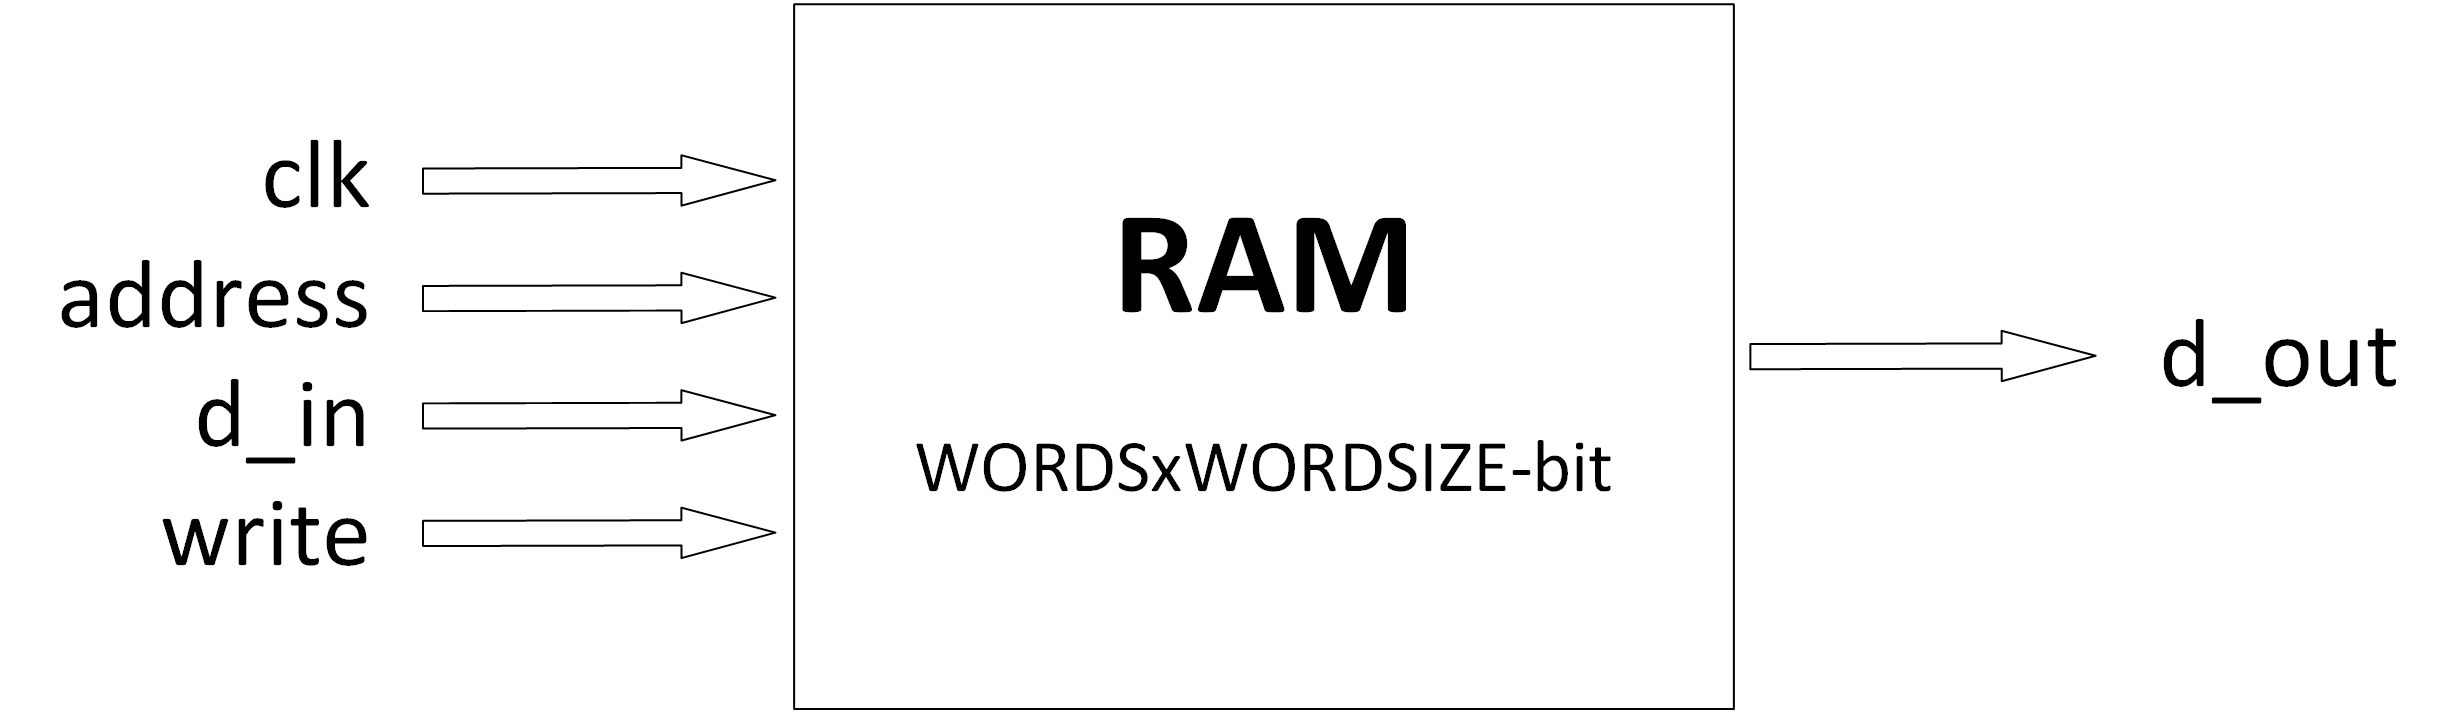
\includegraphics[width=\textwidth]{resource/blackbox-ram}
		\caption{Het blackbox model van ons RAM met de ingangen en uitgangen.}
		\label{fig:blackbox-ram}
\end{figure}
Ons ontwerp is opgedeeld in verschillende blokken omdat onze eerste compleet behavioural beschrijving niet lekker te routen was met een hoge efficientie. Zie figuur \ref{fig:subsystems-ram}.
\begin{figure}[H]
\centering
		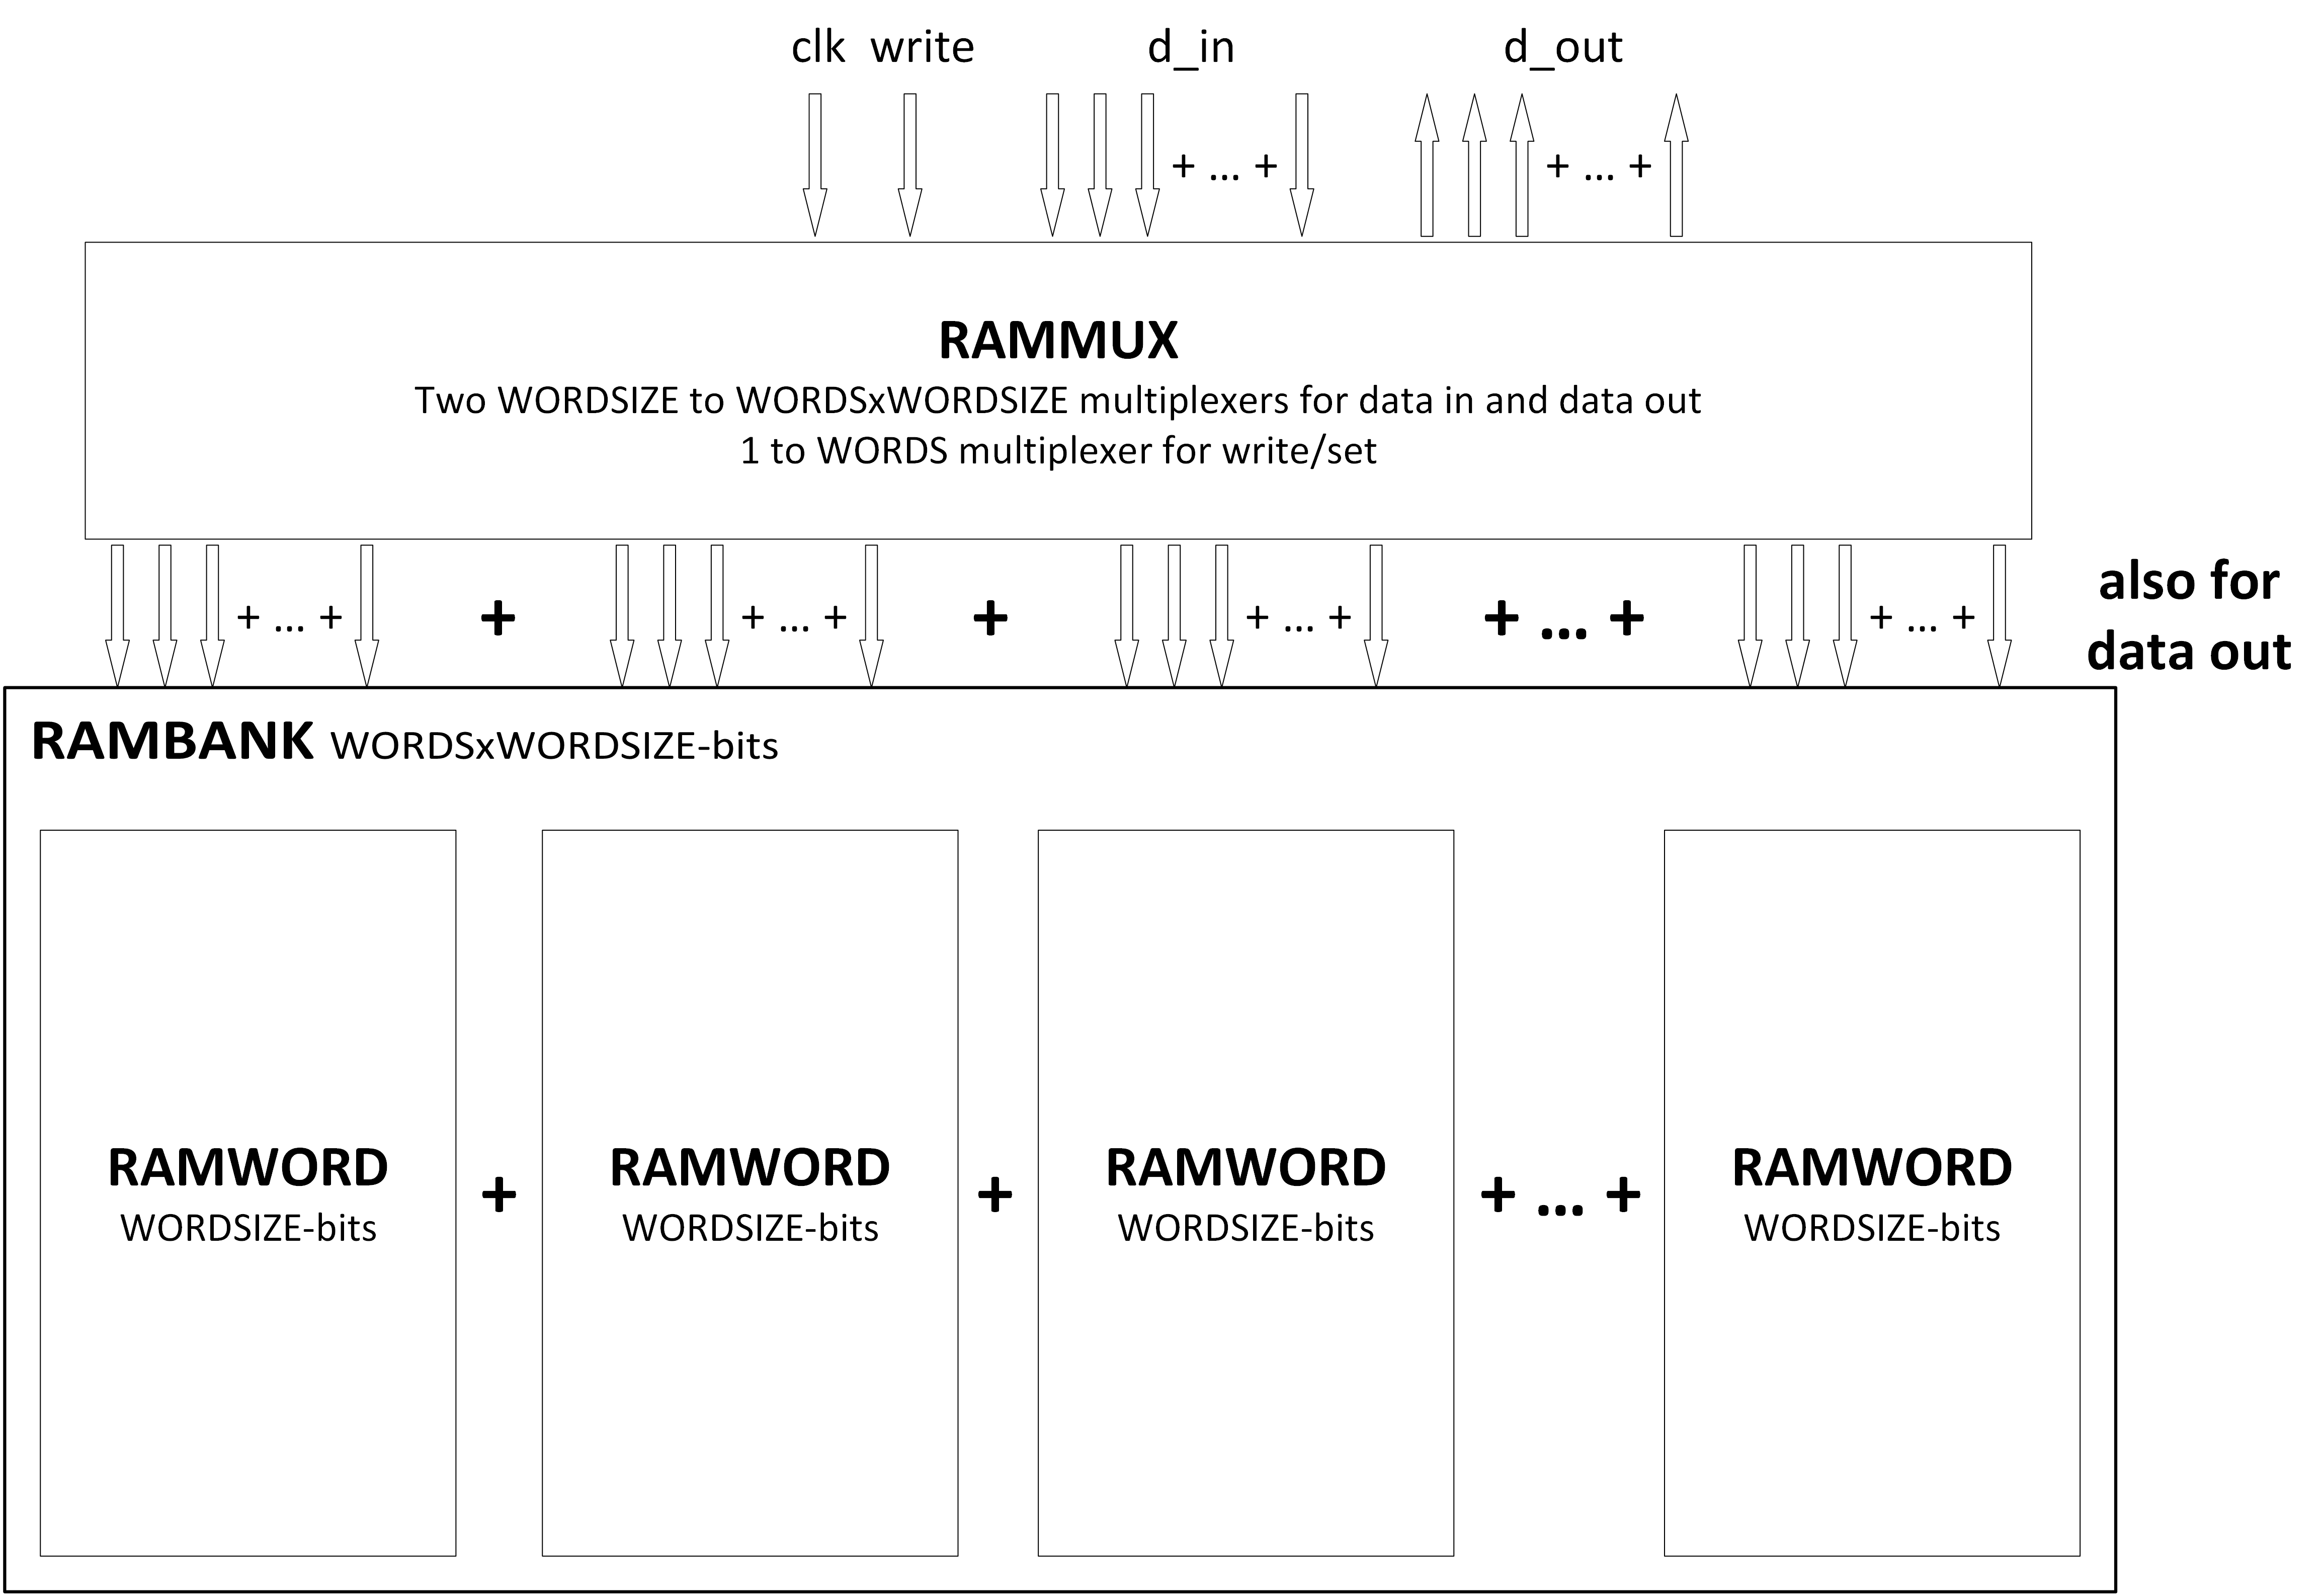
\includegraphics[width=\textwidth]{resource/subsystems-ram}
		\caption{De subsystemen en de sommige tussenverbindingen.}
		\label{fig:subsystems-ram}
\end{figure}
De VHDL implementatie is te zien in \ref{app:ram-vhdl}. De implementatie van onze eerste versie is te zien in \ref{app:b-ram-vhdl}.

%TODO sim results modelsim

\section{Implementatie}
De eerste implementatie hadden we vrij snel klaar. De tweede en meer stucturele hebben we veel langer over gedaan, zelfs zo lang dat we uit eindelijk in tijdnood kwamen. De sysnthse heeft ons veel problemen gegeven vooral de synthese van de grote multiplexers. Maar uit eindelijk hebben we alle gesynthetiseerd gekregen. De layout hebben we waar mogelijk met de hand gedaan. Het routen van de multiplexers naar de rambank gaf het meeste problemen dit is ons uiteindelijk ook niet gelukt.
%TODO switch level sim and layout

\section{Conclusies}
We voldoen volledig eaan de specificaties. De data staat na <10ns stabiel op de uitgang.
We zouden meer aandacht kunnen besteden aan de multiplexer structuul omdat onze rambank op zich zelf heeft een excellente efficientie van 100 procent maar de multiplexer maakte dat het alleen te routen was met een efficientie van rond de 30 procent. Hier kan dus nog aan gewerkt worden.

\newpage
\pagenumbering{Roman}

\printbibliography
\renewcommand{\chapternumber}{\appendixname\;\thechapter}
\begin{appendices}
\section{VHDL implementatie RAM}
\label{app:b-ram-vhdl}
\subsection{ram-pkg.vhd}
\label{appsec:b-ram-pkg.vhd}
\includecode[vhdl]{ram-pkg.vhd}{../../../hardware/opdracht3/ram/VHDL/ram_pkg.vhd}
\subsection{ram.vhd}
\label{appsec:b-ram.vhd}
\includecode[vhdl]{ram.vhd}{../../../hardware/opdracht3/ram/VHDL/ram.vhd}
\subsection{ram-behaviour.vhd}
\label{appsec:b-ram-behaviour.vhd}
\includecode[vhdl]{ram-behaviour.vhd}{../../../hardware/opdracht3/ram/VHDL/ram-behaviour.vhd}

\section{VHDL implementatie RAM2}
\label{app:ram-vhdl}
\subsection{ram-pkg.vhd}
\label{appsec:ram-pkg.vhd}
\includecode[vhdl]{ram-pkg.vhd}{../../../hardware/opdracht3/ram2/VHDL/ram_pkg.vhd}

\subsection{ram.vhd}
\label{appsec:ram.vhd}
\includecode[vhdl]{ram.vhd}{../../../hardware/opdracht3/ram2/VHDL/ram.vhd}

\subsection{ram-behaviour.vhd}
\label{appsec:ram-behaviour.vhd}
\includecode[vhdl]{ram-behaviour.vhd}{../../../hardware/opdracht3/ram2/VHDL/ram-behaviour.vhd}

\subsection{rammux.vhd}
\label{appsec:rammux.vhd}
\includecode[vhdl]{rammux.vhd}{../../../hardware/opdracht3/ram2/VHDL/rammux.vhd}

\subsection{rammux-behaviour.vhd}
\label{appsec:rammux-behaviour.vhd}
\includecode[vhdl]{rammux-behaviour.vhd}{../../../hardware/opdracht3/ram2/VHDL/rammux-behaviour.vhd}

\subsection{rambank.vhd}
\label{appsec:rambank.vhd}
\includecode[vhdl]{rambank.vhd}{../../../hardware/opdracht3/ram2/VHDL/rambank.vhd}

\subsection{rambank-behaviour.vhd}
\label{appsec:rambank-behaviour.vhd}
\includecode[vhdl]{rambank-behaviour.vhd}{../../../hardware/opdracht3/ram2/VHDL/rambank-behaviour.vhd}

\subsection{ramword.vhd}
\label{appsec:ramword.vhd}
\includecode[vhdl]{ramword.vhd}{../../../hardware/opdracht3/ram2/VHDL/ramword.vhd}

\subsection{ramword-behaviour.vhd}
\label{appsec:ramword-behaviour.vhd}
\includecode[vhdl]{ramword-behaviour.vhd}{../../../hardware/opdracht3/ram2/VHDL/ramword-behaviour.vhd}
\end{appendices}
\end{document}